\begin{recipe}
[% 
    preparationtime = {\unit[25]{min}},
    portion = {\portion{4-5}},
    source = {Grandma's love}
]
{Dumplings dough}
    % TODO: vocab: dough
    \introduction{%
        Grandma preparing the dough, children carving out round pieces and modelling the dumplings... that's how home feels like.
    }
    
    \ingredients[4]{%
        \unit[500]{g} & white flour \\
        2   & small eggs \\
        \unit[300]{ml} & warm water \\
        \unit[1]{ts.} & salt
    } 

    \preparation{%
        \step Warm up the water and blend in the eggs. If your eggs are rather large, leave out one yoke.
        
        \step Pug until dry and quite hard. As with pizza dough, you should repeatedly fold in half to get some air bubbles in.
        
        \step Cut into three pieces and cover with a cloth. Roll to about \unit[3]{mm} thick and carve with a thin glass (about \unit[6]{cm} in diameter). 
        
        \step The leftover dough can be gathered after carving and rolled again (once), however do not mix it with the fresh one!
        
        \step Put your favourite stuffing in the middle and stick the edges together. Start in the middle and apply a fair amount of pressure with your fingertips. Make sure the joint is tight!
        
        \step Dumplings should be thrown into large pot with boiling water and boiled for \unit[4-6]{minutes}, depending on the filling. If in doubt, fetch one out and check if the dough is ready in the thickest place.
    }
    
    \hint{%
        If there is a decent amount of leftover dough, roll it once again, cut into 2cm wide stripes and chop these into \unit[1]{mm} wide matches. Dried and boiled these go well with tomato soup.
    }

\end{recipe}


\begin{figure}[h]
    \centering
    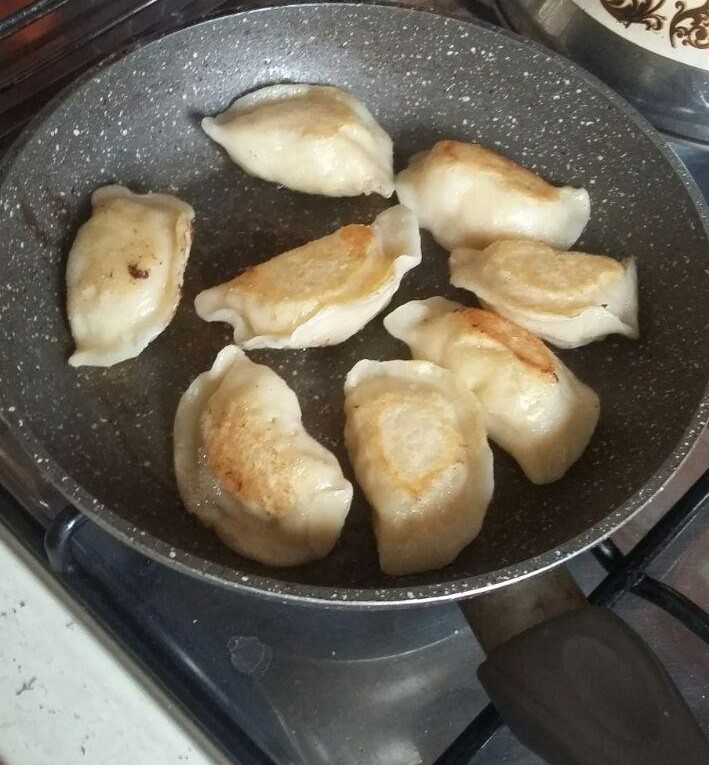
\includegraphics[width=11cm]{pic/dumplings_3}
\end{figure}

\begin{figure}[h]
    \centering
    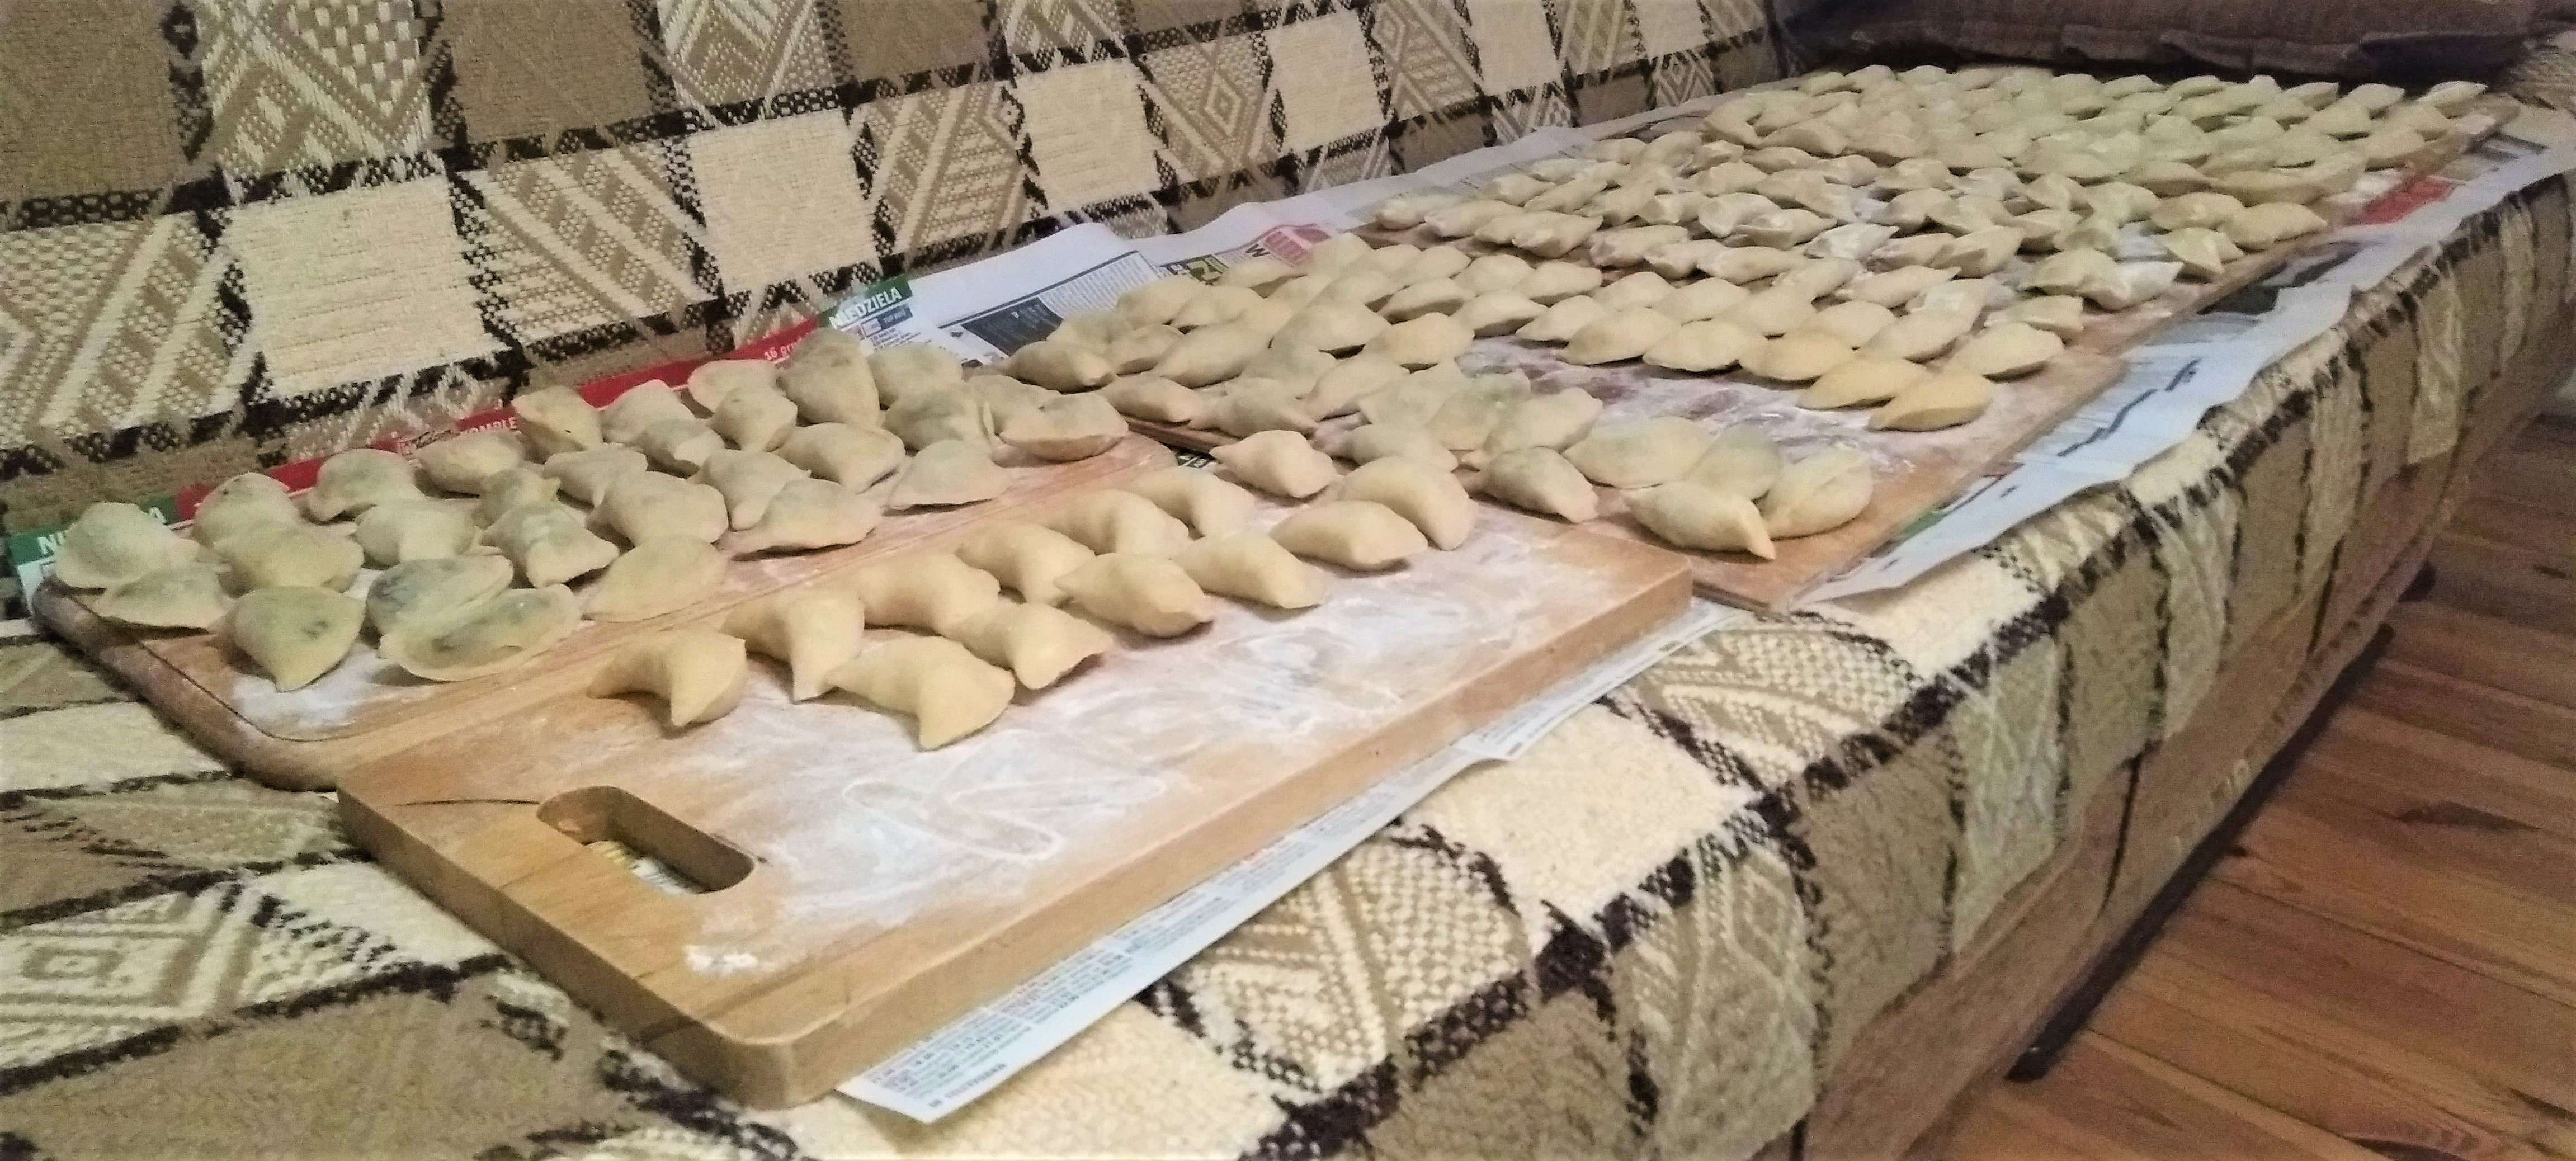
\includegraphics[width=13cm]{pic/dumplings}
\end{figure}
% TODO: alongside